\chapter{Optimal Solution}\label{ch:optimalSolution}
This chapter is meant for framing our take on the best possible hardware and software for us to work (and experiment) with.
The word \textit{optimal} should therefore not be seen as a carefully measured selection of resources, but rather as a greedy pick, had money and time been no problem.
By that logic, anyone referencing this report (perhaps while doing a similar, but more ambitious, project) might find useful suggestions for hardware and software in this chapter.

The chapter ends with a summary of the most essential features of the greedily picked materials, which will help when evaluating the actual hardware and software we will have access to.

\section{Hardware}\label{sec:optimalHardware}
As part of the requirements stated in \autoref{ssec:problemRequirements}, our vehicle should be car-like and host an on-board AV system.
When aiming for a car-like vehicle, some sort of \textit{propulsion} (and steering) is implied, and, to fulfill our requirements for the AV system, some sort of \textit{computing platform} is needed, as well as a \textit{world input}.
All three headlines are further described in this section.

\subsection{Propulsion Platform}\label{ssec:optimalHardwarePropulsion}
A candidate for a combination of chassis, wheels, propulsion, steering, and room for additional hardware, is the \textit{Traxxas TRX-4 Chassis Kit} \cite{TraxxasTRX4}.
\begin{figure}[H]
  \centering
  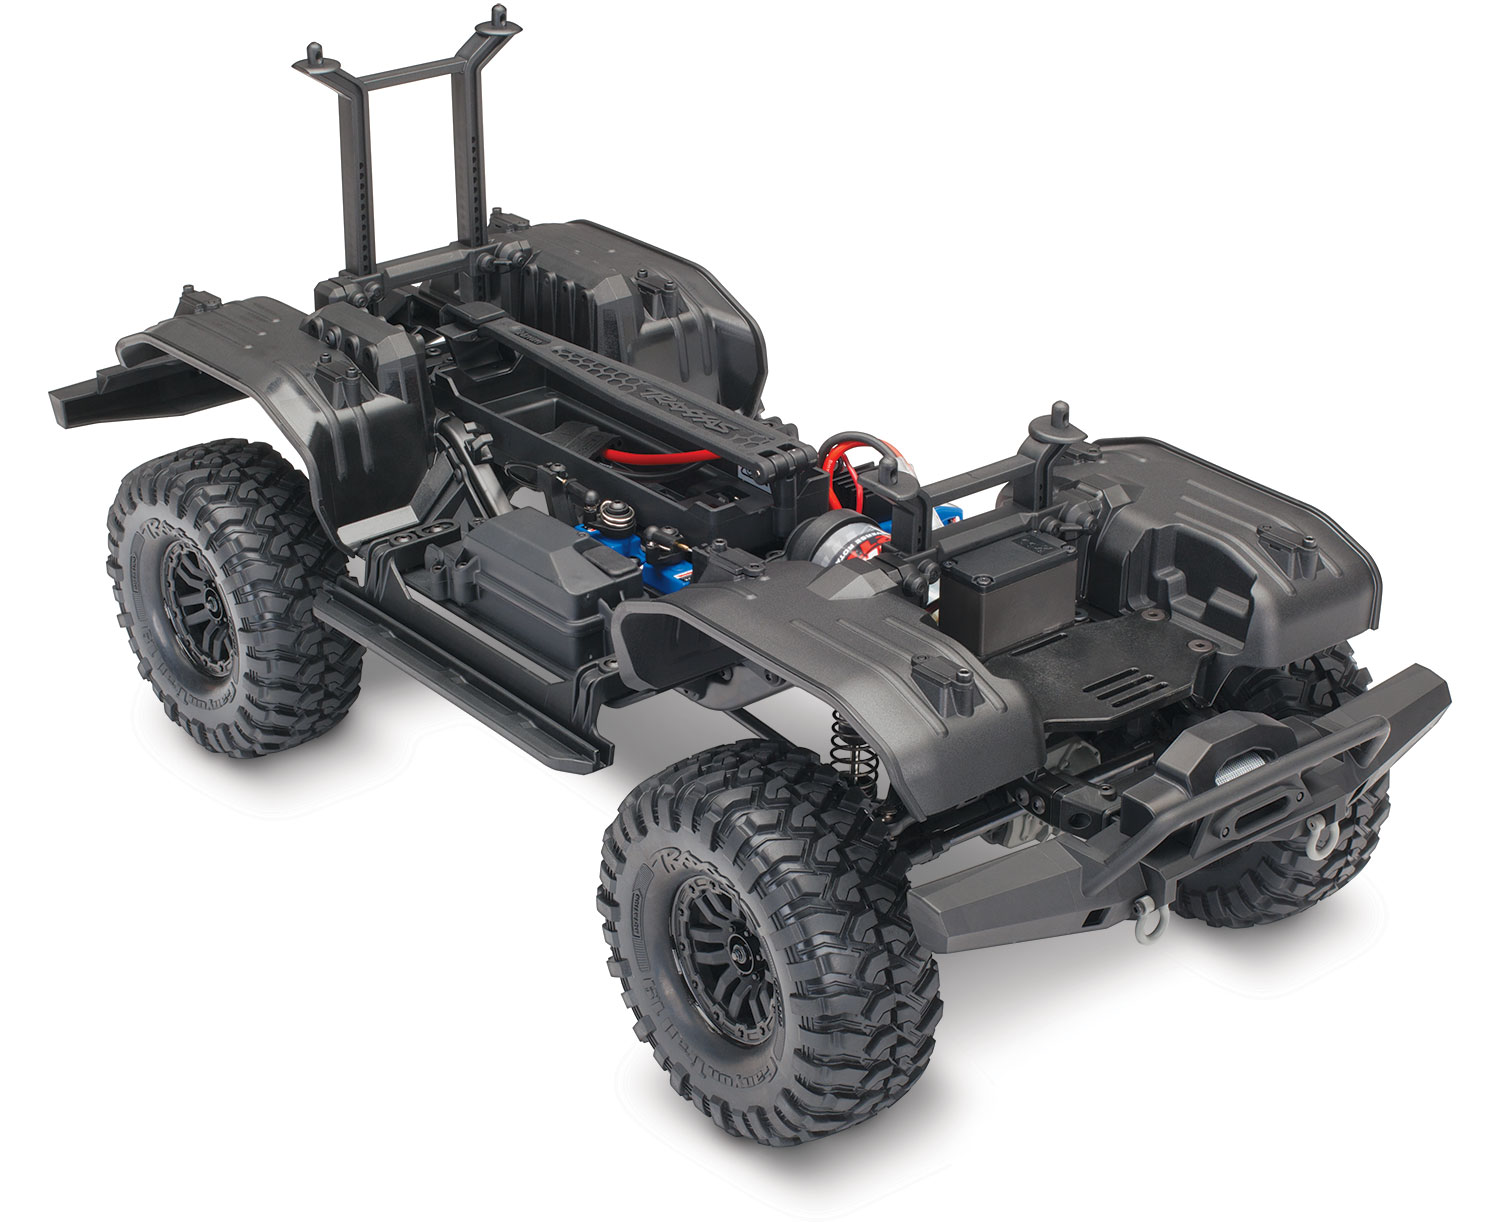
\includegraphics[width=3cm]{images/techAnalysis/TRX4.jpg}
  \caption{Traxxas TRX-4 Chassis Kit}
  \label{fig:TRX4}
\end{figure}
As can be seen on \autoref{fig:TRX4}, this kit provides a minimalistic starting point, allowing as much room as possible for our own additions and adjustments.
All support for wheels, propulsion, and steering would be taken care of with this hardware, as well as any routing of power to, and control of, all motors.
The biggest challenge would be to fit and power our own additional hardware, but, given the minimalism of the chassis, is a problem solvable by 3D-printing the needed brackets/fittings.

\subsection{AV System Platform}\label{ssec:optimalHardwareAVPlatform}
The term "AV System Platform" is, in this section, understood as a link between the engine of the car and the world the car is driving in.
This link is expected to be able to perceive (directly or indirectly) both the world around the car as well as the state of the car itself, make a decision based on all gathered information, and finally have the car perform the requested action.
To accommodate these requirements, the \textit{NVIDIA Jetson Nano Developer Kit} (depicted on \autoref{fig:JetsonNano}) would appear to be a capable platform \cite{JetsonNano}.
\begin{figure}[H]
  \centering
  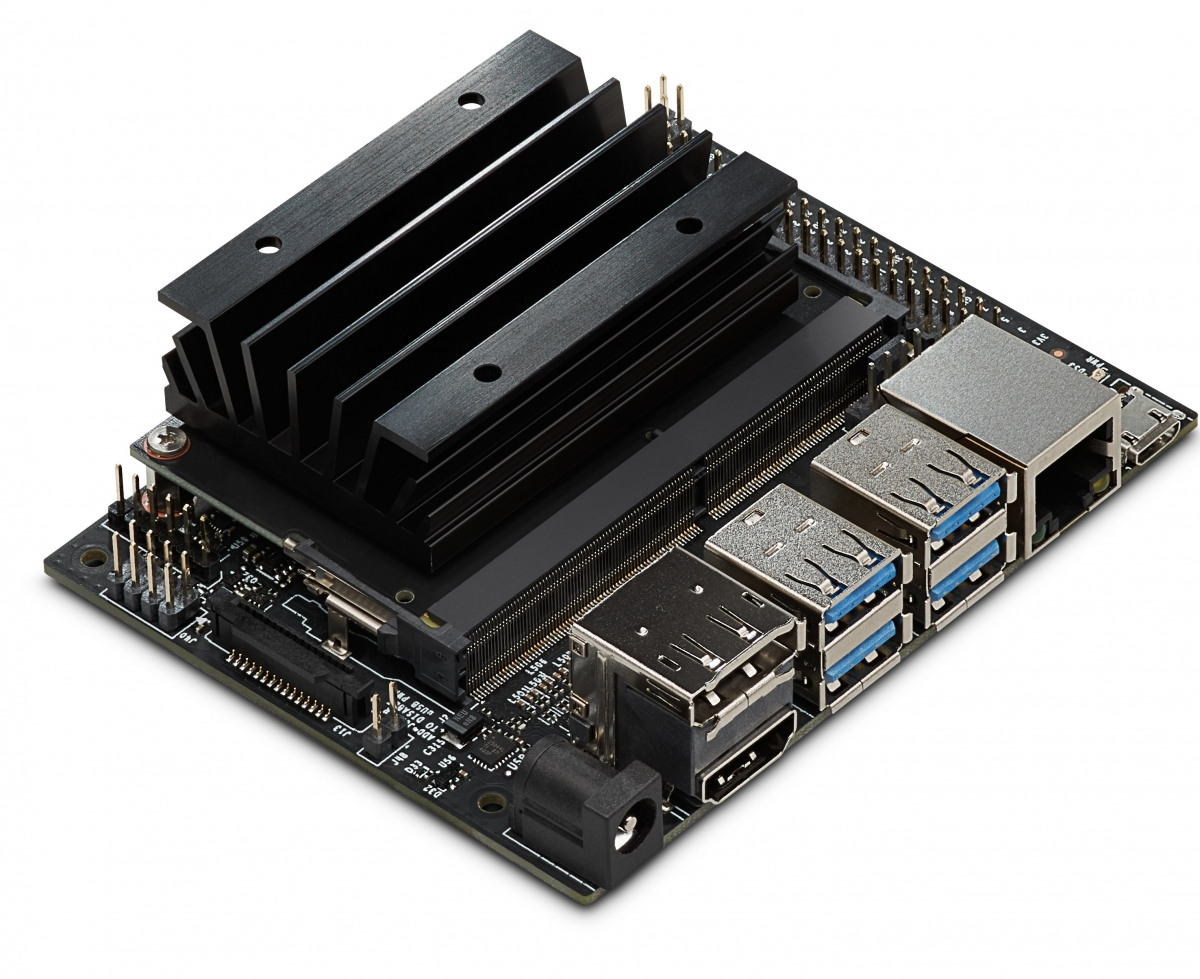
\includegraphics[width=3cm]{images/techAnalysis/JetsonNano.jpg}
  \caption{NVIDIA Jetson Nano Developer Kit}
  \label{fig:JetsonNano}
\end{figure}
As per NVIDIA's own words, the Jetson Nano is ``\textit{[...] a small, powerful computer that lets you run multiple neural networks in parallel for applications like image classification, object detection, segmentation, and speech processing.
All in an easy-to-use platform that runs in as little as 5 watts.}''
The Jetson Nano contains a dedicated 128-core Graphical Processing Unit (GPU) based on the Maxwell architecture, as well as other advantages, making it a powerful starting point.
\cite{JetsonNano}

\subsection{World Input}\label{ssec:optimalHardwareWorldInput}
As for world input to the AV system, not much is required other than ease of use and compatibility.
Since the requirements specifies the need to follow a road represented by colored lines, some sort of camera appears as an obvious candidate.
Any webcam with a USB interface should suffice, and a frequent entry when searching for the ``best USB webcam'' is the \textit{Logitech C922 Pro Stream} \cite{WebcamSearch1, WebcamSearch2, WebcamSearch3} depicted on \autoref{fig:C922}.
\begin{figure}[H]
  \centering
  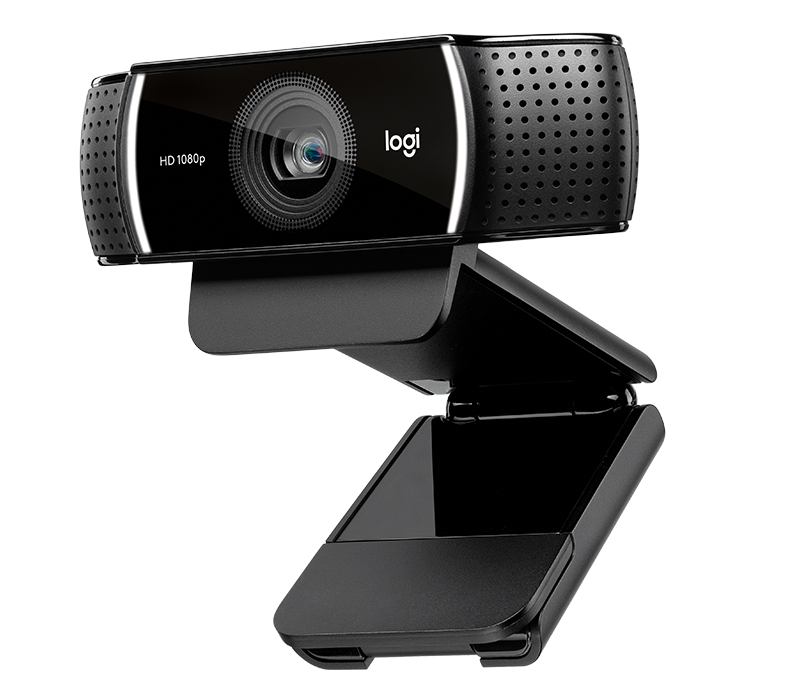
\includegraphics[width=3cm]{images/techAnalysis/c922.png}
  \caption{Logitech C922 Pro Stream}
  \label{fig:C922}
\end{figure}
This webcam is capable of capturing 60 frames per second in a resolution of 1280 times 720 pixels, which should give a satisfying amount of input data for the AV system platform to work with.
As the viewing angle for this camera is 78 degrees, more than one camera could be installed to cover a larger area.

\section{Software}\label{sec:optimalSoftware}
As with the hardware, the choice of software is going to have a significant impact on the final product.
Unlike with the hardware, the software is where we get to do the bulk of the work for this project, and identifying the most optimal choice is therefore not as straight forward.
The following section is one way of answering the question:

The most optimal greedy-choice of software, in terms of delivering something that fulfills our requirements, would be to reuse the software found in existing autonomous vehicles, such as the ones produced by either Google or Tesla mentioned in \autoref{ch:introduction}.
These solutions have already been tried and tested, and should be fairly deploy-able, given the necessary hardware.

The next-most optimal choice of software is going to depend heavily on what hardware is chosen, as not all hardware supports the same software solutions.
If the Jetson Nano from \autoref{ssec:optimalHardwareAVPlatform} was chosen, the obvious choice would be the accompanying \textit{NVIDIA JetPack SDK}, which gives officially supported access to several AI-oriented frameworks, such as \textit{TensorRT} (neural networks) and \textit{OpenCV} (image processing) \cite{JetPack}.

\section{Essential Features}\label{sec:essentialFeatures}
Having looked at the possibilities for choice of hardware and software, the following features from each section will be held in mind when choosing from the provided selection we have access to.

\subsection{Hardware Features}\label{ssec:essentialFeaturesHardware}
A common theme from the hardware described is that they are all designed and pre-built to a point where our job is to do final assembly, and then dive straight into the software design.
This can be seen on the chassis from Traxxas containing all needed components for creating a rough idea of a car, it can be seen on the Jetson Nano being a complete system in itself (with official accompanying operating system and frameworks), and it can be seen on the webcam from Logitech ready to installation via a common USB type A plug.

\subsection{Software Features}\label{ssec:essentialFeaturesSoftware}
The software had two common themes worth mentioning: reuse of existing solutions, and easily accessible tools for building a new solution.

Given the needed hardware, we acknowledge the existence of solutions made with both scientific and commercial goals, and deploying those would indeed get us to the finish line for this project.

By taking the suggested Jetson Nano into account, and thereby making the hardware the limiting factor (instead of the software), the choice points more in the direction of pre-built frameworks and tools for us to experiment and work with.

